\documentclass[11pt,a4paper]{article}
\usepackage[margin=2.2cm]{geometry}
\usepackage{amsmath,amssymb,amsthm,bm}
\usepackage{graphicx,booktabs,multirow,xcolor}
\usepackage{algorithm,algpseudocode}
\usepackage{listings}
\usepackage{microtype}
\usepackage[numbers,sort&compress]{natbib}
\usepackage[colorlinks=true,linkcolor=blue!50!black,citecolor=blue!50!black,urlcolor=blue!50!black]{hyperref}
\usepackage{cleveref}

\lstset{basicstyle=\ttfamily\small,keywordstyle=\color{blue!60!black}\bfseries,commentstyle=\color{gray},
  language=Python,frame=single,breaklines=true,columns=fullflexible,captionpos=b}
\newcommand{\R}{\mathbb{R}}
\newtheorem{proposition}{Proposition}

\title{Fading Memory: Where State-Space Models Fail on Recall and State Tracking,\\ and What Fixes Them}
\author{Devansh \\ Roll No.\ \underline{\hspace{3cm}} \\[2pt] EE798R Pattern Recognition --- Course Project}
\date{\today}

\begin{document}
\maketitle
\begin{abstract}
Linear-time recurrent sequence models such as Mamba-2 and Gated DeltaNet are replacing most attention
layers in recent large language models because they keep a fixed-size state instead of a key--value cache
that grows with the context. This report studies what that \emph{fading memory} costs and what it buys.
We implement, from scratch, a selective state-space model (SSM), Gated DeltaNet and a Transformer baseline,
each with a reference recurrence and a verified chunkwise-parallel training algorithm, plus two recent
extensions: a rotational (complex-valued, Mamba-3-style) SSM and DeltaProduct. All models are trained on a
single RTX~4050 laptop GPU on synthetic pattern-recognition probes: state tracking in the groups
$\mathbb{Z}_2$, $\mathbb{Z}_3$ and $S_3$ with length generalisation, and multi-query associative recall.
Three results stand out. (i) Allowing negative eigenvalues makes the SSM solve parity at 8$\times$ the
training length (0.999 vs.\ 0.546). (ii) DeltaProduct, a product of two generalised Householder
reflections per token, is the only model that learns the non-abelian group $S_3$ on all seeds and keeps
0.912 accuracy at 8$\times$ the training length, versus 0.542 for Gated DeltaNet. (iii) Recall degrades
exactly when the number of stored pairs outgrows the recurrent state, while Gated DeltaNet stores 64 pairs
with half the state of an SSM that fails. We also document failures: models that fit the training length
perfectly but learn shortcuts, a rotational SSM that can represent $\mathbb{Z}_3$ but does not learn it
(confirmed by reading its angles from the weights), and an under-budgeted recall sweep that ranked models
wrongly. A GPU study shows that, at feasible lengths, kernel quality dominates asymptotic complexity.
\end{abstract}

\section{Introduction and Motivation}
\label{sec:intro}

Self-attention \citep{vaswani2017attention} compares every token with every earlier token. This gives the
Transformer an exact, content-addressable memory of its entire context, but at a price: training costs
$O(T^2)$ time in the sequence length $T$, and generation must keep a key--value (KV) cache whose size
grows linearly with the context. For long contexts the KV cache, not the arithmetic, becomes the
bottleneck of deployment.

A family of \emph{linear recurrent} sequence models removes this cost. State-space models (SSMs) such as
Mamba \citep{gu2023mamba} and Mamba-2 \citep{dao2024ssd}, and linear-attention models such as Gated
DeltaNet \citep{yang2025gated}, compress the whole past into a state of fixed size, updated once per token.
Training runs in $O(T)$ with a parallel scan, and generation needs constant memory per sequence. These
layers are no longer a research curiosity: recent production models are hybrids that replace most of
their attention layers with them, for example Kimi Linear \citep{kimi2025linear}, which interleaves three
delta-rule layers with every attention layer.

The price of a fixed-size state is that the memory must \emph{fade}: information is compressed, decayed
and overwritten. Which pattern-recognition abilities survive this compression, and which do not, is the
question of this project. Two abilities are particularly revealing.
\begin{itemize}
  \item \textbf{Associative recall}: storing many key--value facts and retrieving one by its key. Attention
        does this by direct lookup; a recurrent model must fit all facts into its state.
  \item \textbf{State tracking}: maintaining a running summary that changes with every input, such as the
        parity of a bit string or the composition of a sequence of permutations. Here the question is not
        how much the state can hold, but which updates the recurrence can express at all.
\end{itemize}
Both are pattern-recognition problems in the classical sense: a sequence must be mapped to a label, and
the model must discover a rule from examples rather than memorise them. We probe them with controlled
synthetic tasks, which isolate a single ability and allow testing on sequences longer than any seen in
training, the cleanest check that a rule rather than a shortcut was learned.

\paragraph{Research questions.}
\begin{enumerate}
  \item[\textbf{RQ1}] How much associative recall can a fixed-size state support, and how does this depend
        on the size of the state and on the update rule?
  \item[\textbf{RQ2}] Which state transitions can track state? We test parity ($\mathbb{Z}_2$), counting
        modulo 3 ($\mathbb{Z}_3$) and the non-abelian permutation group $S_3$, the negative-eigenvalue fix
        of \citet{grazzi2025unlocking}, and two recent extensions: complex-valued (rotational) transitions
        in the spirit of Mamba-3 \citep{mamba3} and products of Householder matrices
        (DeltaProduct, \citealp{siems2025deltaproduct}).
  \item[\textbf{RQ3}] What does the linear-time recurrence buy in latency and memory on a consumer GPU, and
        how much does the quality of the GPU kernel matter?
\end{enumerate}

\paragraph{Contributions.}
\begin{itemize}
  \item From-scratch implementations of a selective SSM, Gated DeltaNet, a rotational SSM, DeltaProduct
        and a Transformer baseline. Each recurrent mixer has a token-by-token reference and a
        chunkwise-parallel training algorithm, verified against each other to float64 precision, and
        constant-memory decoding verified against the parallel forward pass.
  \item A Triton GPU kernel for the SSM scan and an efficiency study on an RTX~4050 laptop GPU.
  \item A controlled comparison on state tracking (8 models $\times$ 3 groups $\times$ 3 seeds) and
        associative recall, all on one 6\,GB GPU.
  \item An analysis of four failure cases, including a direct inspection of learned weights showing that a
        model which \emph{can} represent the solution learned a shortcut instead.
\end{itemize}

\paragraph{Scope.} All experiments use small models (0.2--0.44M parameters, two layers) on synthetic
tasks. The aim is not state-of-the-art accuracy but a clean, mechanistic comparison whose conclusions can
be traced back to the mathematics of each recurrence.

\section{Background and Related Work}
\label{sec:background}

\paragraph{From attention to linear recurrences.} Softmax attention computes, for every query, a
normalised weighting over all previous keys \citep{vaswani2017attention}. \citet{katharopoulos2020transformers}
observed that replacing the softmax kernel by a feature-map dot product turns causal attention into a
recurrence: the sum $\sum_j \phi(k_j) v_j^\top$ can be accumulated token by token in a matrix-valued state,
so a Transformer becomes an RNN with $O(1)$ cost per token. \citet{schlag2021linear} interpreted this state
as a set of \emph{fast weights} written by the network itself, and pointed out its weakness: purely
additive writes cannot overwrite old associations, so the memory fills up with interference. This
observation motivates the delta rule discussed below.

\paragraph{Structured and selective state-space models.} SSMs start from a continuous linear system
$\dot h = Ah + Bx$, $y = Ch$, discretised in time. S4 \citep{gu2022s4} made such models trainable on long
sequences by structuring $A$ and computing the output as a long convolution, which requires the system to
be time-invariant. Mamba \citep{gu2023mamba} gave up time invariance: the step size $\Delta_t$ and the
matrices $B_t, C_t$ depend on the current input, so the model can decide what to store and what to forget
(\emph{selectivity}). The price is that the convolution view is lost and a scan is needed. Mamba-2
\citep{dao2024ssd} restricted $A$ to a scalar per head and showed that the resulting model is exactly a
form of masked linear attention (\emph{state-space duality}), which yields a chunkwise algorithm built from
matrix multiplications. Mamba-3 \citep{mamba3} adds a more accurate (trapezoidal) discretisation,
complex-valued state transitions, which it shows are equivalent to a data-dependent rotary embedding, and a
multi-input multi-output form designed for fast inference. This project implements the Mamba-2 recurrence
and a rotational variant inspired by Mamba-3.

\paragraph{Delta-rule models.} DeltaNet replaces the additive write of linear attention with the delta
rule: before writing a value under a key, it first removes what the memory currently returns for that
key. \citet{yang2024deltanet} made this trainable at scale with a chunkwise algorithm based on a compact
representation of products of Householder-like matrices. Gated DeltaNet \citep{yang2025gated} adds a
Mamba-2-style decay gate, so the model can both overwrite precisely and forget globally. Kimi Delta
Attention \citep{kimi2025linear} refines the gate to be channel-wise and is deployed in a 48B-parameter
hybrid model.

\paragraph{What fixed-size memories cannot do.} Two lines of work characterise the limits of these
models, and they correspond to the two abilities studied here. For \emph{recall}, \citet{arora2024zoology}
introduced the multi-query associative recall (MQAR) task and showed that the gap between efficient models
and attention in language modelling is largely explained by recall; \citet{jelassi2024repeat} proved and
showed empirically that Transformers copy long strings that fixed-state models cannot; and
\citet{michalak2025some} found that in hybrid production models retrieval is carried entirely by the
attention layers. For \emph{state tracking}, \citet{merrill2024illusion} argued that diagonal SSMs, like
Transformers, cannot express inherently sequential computations such as composing permutations.
\citet{grazzi2025unlocking} identified a simple culprit: transition eigenvalues restricted to $[0,1]$ make
even parity impossible, and extending them to $[-1,1]$ fixes parity for Mamba and DeltaNet. DeltaProduct
\citep{siems2025deltaproduct} goes further by applying several Householder steps per token, which can
represent rotations and general permutations.

\paragraph{Where this project sits.} Prior studies typically examine one model family and one ability.
Here the three families (attention, diagonal SSMs, delta-rule models) share one codebase, one training
protocol and one GPU, and are tested on both abilities. This makes the comparison controlled: differences
can be attributed to the recurrence itself. We reproduce the negative-eigenvalue result, extend it to
rotations and Householder products, and report where each mechanism stops working. The conclusion
of \citet{yu2025mambaout}, that Mamba is unnecessary for short, non-sequential vision tasks, is consistent
with our framing: the recurrence matters precisely for long, sequential problems.

\section{Theory and Conceptual Explanation}
\label{sec:theory}
% Guideline 2.4: intuition, assumptions, architecture, design choices, advantages, limitations. Diagrams!

\todo{Figure: one block of each mixer (attention / selective SSM / Gated DeltaNet) side by side.}

\paragraph{Two kinds of memory.} \todo{Attention = exact, growing, content-addressable memory.
Recurrent mixer = fixed-size summary updated online. Intuition for why recall degrades once the
number of stored facts exceeds what the state can hold.}

\paragraph{Selectivity.} \todo{Why input-dependent $\Delta_t$, $B_t$, $C_t$ let the SSM choose what to
store and what to forget (needed for selective copying).}

\paragraph{The delta rule as online regression.} \todo{Erase-then-write: the state behaves as a
key--value memory updated by one gradient step on $\tfrac12\lVert S^\top k_t - v_t\rVert^2$.}

\paragraph{Why eigenvalues matter for state tracking.} \todo{Parity needs a sign flip; decays in
$(0,1)$ can only shrink. Rotations for $\mathbb{Z}_m$; non-diagonal transitions for $S_3$.}

\paragraph{Advantages and limitations.} \todo{Linear time, constant-memory decoding vs.\ lossy recall,
restricted expressivity, sensitivity to hyperparameters.}

\section{Mathematical Formulation}
\label{sec:math}
% Guideline 2.5 (mandatory): define every symbol; derive, don't copy.
% The equations below match the code exactly; rewrite the surrounding explanation in your own words.

\subsection{Task as a sequence-labelling problem}
A model $f_\theta$ maps a token sequence $x_{1:T}$ to per-position distributions over a vocabulary
$\mathcal{V}$. With a mask $m_t\in\{0,1\}$ marking scored positions, training minimises
\begin{equation}
  \mathcal{L}(\theta) = -\frac{1}{\sum_{n,t} m^{(n)}_t}\sum_{n=1}^{N}\sum_{t=1}^{T} m^{(n)}_t
  \log p_\theta\!\left(y^{(n)}_t \mid x^{(n)}_{1:t}\right).
\end{equation}
\todo{Explain $N$, $y_t$, the causal conditioning, and why only masked positions count.}

\subsection{Causal softmax attention}
\begin{equation}
  o_t = \sum_{j\le t} \frac{\exp(q_t^\top k_j/\sqrt{d})}{\sum_{i\le t}\exp(q_t^\top k_i/\sqrt{d})}\, v_j .
\end{equation}
\todo{Cost $O(T^2 d)$ for training; decoding reads a KV cache of $2Td$ numbers per layer and head.}

\subsection{Selective state-space model}
Continuous-time system $\dot h(\tau) = A h(\tau) + B x(\tau)$, $y = C h$. Zero-order-hold
discretisation with an input-dependent step $\Delta_t$ and scalar $A=-e^{\alpha}<0$ per head gives
\begin{align}
  a_t &= \exp(\Delta_t A) \in (0,1), \qquad \Delta_t = \operatorname{softplus}(w^\top u_t + b),\\
  h_t &= a_t\, h_{t-1} + (\Delta_t x_t)\, B_t^\top, \qquad h_t \in \R^{P\times N},\\
  y_t &= h_t C_t + D x_t .
\end{align}
\todo{Define $P$ (head channels), $N$ (state size), $B_t, C_t\in\R^N$. Explain the Euler-style
approximation of the input term used by Mamba-2 and what Mamba-3's trapezoidal rule changes.}

\paragraph{Unrolled (dual) form.} Unrolling the recurrence,
\begin{equation}
  y_t = \sum_{j\le t} \underbrace{\Big(\prod_{k=j+1}^{t} a_k\Big)}_{\text{decay mask } L_{tj}}
        (C_t^\top B_j)\, \Delta_j x_j ,
\end{equation}
i.e.\ causal attention with scores $C_t^\top B_j$ and a multiplicative decay mask \citep{dao2024ssd}.
\todo{Derive this by induction.}

\paragraph{Chunkwise algorithm.} \todo{Split $T$ into chunks of length $L$. Within a chunk use the dual
form ($O(L^2)$); across chunks carry $h$ with one recurrence step per chunk. Total cost
$O(T L N P)$; show the three terms (intra-chunk output, chunk state, inter-chunk contribution) and how
negative $a_k$ are handled via $\log|a_k|$ and a sign product.}

\paragraph{Negative eigenvalues.} With $a_t\mapsto 2a_t-1\in(-1,1)$ the state can flip sign.
\todo{Prove: a 1-D state with $a_t=-1$ on input 1 and $a_t=1$ on input 0 computes parity; with
$a_t\in(0,1)$ the sign of $h_t$ can never alternate (sketch of \citet{grazzi2025unlocking}).}

\subsection{Gated delta rule}
With $\alpha_t\in(0,1]$, $\beta_t\in(0,1)$ (or $(0,2)$) and $\lVert k_t\rVert=1$,
\begin{align}
  S_t &= \alpha_t\,(I - \beta_t k_t k_t^\top)\, S_{t-1} + \beta_t\, k_t v_t^\top, \qquad S_t\in\R^{d_k\times d_v},\\
  o_t &= S_t^\top q_t .
\end{align}
\todo{Show this is one SGD step (learning rate $\beta_t$) on $\tfrac12\lVert S^\top k_t - v_t\rVert^2$
after decaying by $\alpha_t$. Eigenvalues of $I-\beta_t k_t k_t^\top$: $1-\beta_t$ along $k_t$ and 1
elsewhere.}

\paragraph{Chunkwise (UT-transform) form.} Let $\gamma_i=\sum_{k\le i}\log\alpha_k$ inside a chunk and
$\Gamma_i = e^{\gamma_i}$. The vectors actually written, $u_i=\beta_i(v_i-\alpha_i S_{i-1}^\top k_i)$,
solve the unit lower-triangular system
\begin{equation}
  (I+M)\,U = \operatorname{diag}(\beta)\,V - \operatorname{diag}(\beta\odot\Gamma)\,K S_0, \qquad
  M_{ij} = \beta_i\, e^{\gamma_i-\gamma_j}\, k_i^\top k_j \ (j<i),
\end{equation}
after which $O = (Q\odot\Gamma)S_0 + (QK^\top\odot \mathcal{D})\,U$ with decay mask
$\mathcal{D}_{ij}=e^{\gamma_i-\gamma_j}\mathbb{1}[j\le i]$. \todo{Derive; complexity.}

\subsection{State-tracking as group products}
\todo{Define the word problem: $y_t = g_1 g_2\cdots g_t$ for $g_i$ in a finite group $G$. Parity:
$G=\mathbb{Z}_2$; $\mathbb{Z}_m$ needs rotations; $S_3$ is non-abelian. Relate to which transition
matrices can represent $G$.}

\subsection{Complexity summary}
\begin{table}[h]\centering
\begin{tabular}{lccc}\toprule
Mixer & Training time & Decode time / token & Decode memory \\\midrule
Attention & $O(T^2 d)$ & $O(T d)$ & $O(T d)$ \\
Selective SSM (chunked) & $O(T L N P)$ & $O(NP)$ & $O(NP)$ \\
Gated DeltaNet (chunked) & $O(T (L d + d^2))$ & $O(d^2)$ & $O(d^2)$ \\\bottomrule
\end{tabular}
\caption{Per-layer, per-head cost. $L$ = chunk length. \todo{check and explain}}
\end{table}

\section{Algorithm and Methodology}
\label{sec:method}
% Guideline 2.6: inputs/outputs, preprocessing, features, architecture, training, inference, hyperparameters.

\paragraph{Model.} Token embedding $\rightarrow$ $n$ pre-norm residual blocks (RMSNorm, mixer,
optional SwiGLU MLP) $\rightarrow$ RMSNorm $\rightarrow$ tied output head. The mixer of each layer is set by
a pattern string (\texttt{A}/\texttt{M}/\texttt{D}), e.g.\ \texttt{MAMM}.

\begin{algorithm}[h]
\caption{Chunkwise selective scan (training)}
\begin{algorithmic}[1]
\Require $x\in\R^{T\times H\times P}$, $a\in\R^{T\times H}$, $B,C\in\R^{T\times N}$, chunk length $L$
\State Pad $T$ to a multiple of $L$ with $a=1$, $x=B=C=0$
\For{each chunk $c$ (in parallel)}
  \State $\ell_i \gets \sum_{k\le i}\log|a_k|$, \ $s_i \gets \prod_{k\le i}\operatorname{sgn}(a_k)$
  \State $Y^{\text{diag}}_c \gets \big((C B^\top)\odot \mathcal{L}\big)\, x$ \Comment{$\mathcal{L}_{ij}=s_is_je^{\ell_i-\ell_j}[j\le i]$}
  \State $\Sigma_c \gets \sum_j s_Ls_j e^{\ell_L-\ell_j} x_j B_j^\top$
\EndFor
\For{$c = 1,\dots,T/L$ (sequential)} \State $h_c \gets h_{c-1}$ decayed over chunk $c-1$ $+\ \Sigma_{c-1}$ \EndFor
\State $Y \gets Y^{\text{diag}} + \big(s_i e^{\ell_i}\big) \cdot C\,h_c$
\end{algorithmic}
\end{algorithm}

\paragraph{Training.} \todo{AdamW, warmup + cosine, gradient clipping, bf16 autocast, infinite freshly
sampled data, early stopping at 99.5\% (MQAR), learning-rate grid per architecture.}

\paragraph{Inference.} \todo{Parallel forward for evaluation; recurrent \texttt{step()} for decoding
with constant state (SSM, DeltaNet) vs.\ KV cache (attention).}

\section{Implementation and Code Snippets}
\label{sec:impl}

All models, tasks and kernels were implemented for this project in PyTorch and Triton
\citep{tillet2019triton}; no external state-space or linear-attention library is used. The code is available
at \url{https://github.com/Devx228/EE798-project}. The main files are \texttt{layers/ssm.py} (selective and
rotational SSM), \texttt{layers/deltanet.py} (Gated DeltaNet and DeltaProduct), \texttt{layers/attention.py},
\texttt{layers/triton\_scan.py}, \texttt{tasks/} (data generators), \texttt{train.py} and the experiment
scripts. The code was written with the help of an AI coding assistant; the experiments were run on the
author's own GPU, and all reported numbers come from those runs.

\paragraph{Reference recurrence.} Listing~\ref{lst:delta} is the token-by-token form of
\eqref{eq:delta}. It is slow, but it is the ground truth for testing the chunked algorithm.
\begin{lstlisting}[caption={Reference gated delta rule (\texttt{layers/deltanet.py}).},label={lst:delta}]
for t in range(T):
    S = S * torch.exp(g[:, :, t])[..., None, None]          # decay: alpha_t * S
    v_old = torch.einsum("bhkv,bhk->bhv", S, k[:, :, t])    # what memory returns for k_t
    S = S + torch.einsum("bhk,bhv->bhkv", k[:, :, t],
                         beta[:, :, t, None] * (v[:, :, t] - v_old))  # erase + write
    outs.append(torch.einsum("bhkv,bhk->bhv", S, q[:, :, t]))         # o_t = S^T q_t
\end{lstlisting}
The first line applies the decay $\alpha_t=e^{g_t}$ to the whole state. The second reads the value currently
stored under the key, $S^\top k_t$. The third adds $\beta_t k_t(v_t-S^\top k_t)^\top$, which is the
gradient step of Section~\ref{sec:math}: with $\beta_t=1$ the old value is fully replaced. The last line
reads the memory with the query.

\paragraph{Changing the eigenvalue range.} The negative-eigenvalue variant is a one-line change after the
discretisation \eqref{eq:disc} (Listing~\ref{lst:neg}); for DeltaNet the analogous change is
\texttt{beta = 2 * beta}.
\begin{lstlisting}[caption={Decay of the selective SSM (\texttt{layers/ssm.py}).},label={lst:neg}]
dt = F.softplus(dt_raw + self.dt_bias)        # step size Delta_t > 0
a = torch.exp(-dt * torch.exp(self.A_log))    # a_t = exp(Delta_t * A), A < 0, so a_t in (0, 1)
if self.neg_eigen:
    a = 2.0 * a - 1.0                         # a_t in (-1, 1): the state can flip sign
\end{lstlisting}

\paragraph{Rotations as a data-dependent RoPE.} Equation \eqref{eq:rope} is implemented literally: the
cumulative angle is a prefix sum, $B$ and $C$ are rotated by it, and the verified real scan does the rest.
\begin{lstlisting}[caption={Rotational SSM (\texttt{layers/ssm.py}).},label={lst:rot}]
def rotational_scan(x, a, theta, B, C, chunk_size=64):
    phase = theta.cumsum(dim=1)                       # Phi_t = sum_{k<=t} theta_k
    return ssd_scan_chunked(x, a, rotate_pairs(B, -phase), rotate_pairs(C, -phase), chunk_size)
\end{lstlisting}

\paragraph{DeltaProduct by interleaving.} Rather than writing a new kernel, the $n_h$ Householder steps of
\eqref{eq:product} are laid out along the time axis: token $t$, sub-step $j$ becomes position $tn_h+j$.
The decay is applied only at the first sub-step and the query only at the last, so the verified chunked
delta rule computes DeltaProduct exactly.
\begin{lstlisting}[caption={DeltaProduct via interleaving (\texttt{layers/deltanet.py}).},label={lst:prod}]
q_x = q.new_zeros(b, T, n_h, H, d); q_x[:, :, -1] = q   # read memory after the last sub-step
g_x = g.new_zeros(b, T, n_h, H);    g_x[:, :, 0] = g    # decay once per token
o, S = delta_rule_chunked(*flatten(q_x, k, v, beta, g_x))  # sequence of length T * n_h
o = o[:, :, n_h - 1 :: n_h]                               # one output per token
\end{lstlisting}

\paragraph{Triton scan kernel.} Listing~\ref{lst:triton} is the inner loop of the forward kernel. One GPU
program handles one (sequence, head, block of $P$ channels) and keeps its $[B_P\times N]$ slice of the state
in registers for the whole sequence, so the state never travels to global memory; only $x,a,B,C$ are read
and $y$ is written.
\begin{lstlisting}[caption={Inner loop of the Triton scan kernel (\texttt{layers/triton\_scan.py}).},label={lst:triton}]
state = tl.zeros([BLOCK_P, BLOCK_N], dtype=tl.float32)
for t in range(T):
    a_t = tl.load(a_base + t * s_at)
    x_t = tl.load(x_base + t * s_xt, mask=mask_p, other=0.0)
    b_t = tl.load(b_base + t * s_bt, mask=mask_n, other=0.0)
    c_t = tl.load(c_base + t * s_ct, mask=mask_n, other=0.0)
    state = a_t * state + x_t[:, None] * b_t[None, :]     # h_t = a_t h_{t-1} + x_t B_t^T
    y_t = tl.sum(state * c_t[None, :], axis=1)             # y_t = h_t C_t
    tl.store(y_base + t * s_yt, y_t, mask=mask_p)
\end{lstlisting}

\paragraph{Data generation.} The MQAR generator writes $n$ key--value pairs at the start of the sequence and
places each key once more as a query at a random later position, followed by its value; only query positions
are scored. Keys are drawn without replacement from the lower half of the vocabulary and values from the
upper half. The group-word generator samples uniform group elements and computes prefix products with a
precomputed multiplication table (for $S_3$, the composition table of all six permutations).

\paragraph{Verification.} A test suite (62 tests on the CPU plus the Triton kernel tests on the GPU) checks that (i) every chunked algorithm (SSM with positive
and negative decays, rotational SSM, gated delta rule with $\beta\in(0,2)$, DeltaProduct) matches its
token-by-token reference in float64 (maximum error $\approx10^{-15}$) for sequence lengths that are and are not
multiples of the chunk length; (ii) the single-token decoding of every model reproduces its parallel forward
pass; (iii) the Triton kernel matches the reference (run on the GPU, and on CPU in Triton's interpreter mode);
and (iv) the task generators produce correct labels and the group tables satisfy the group axioms. Two
further tests check the algebra behind the extensions: a rotation by $2\pi/3$ returns the state after three
steps, and the product of two reflections is a rotation of order three when the keys are $60^\circ$ apart.

\section{Dataset and Experimental Setup}
\label{sec:setup}

\paragraph{Tasks.} All data are synthetic and generated on the fly; no external dataset is used.
\begin{itemize}
  \item \textbf{Group word problems (RQ2).} Groups $\mathbb{Z}_2$ (2 tokens), $\mathbb{Z}_3$ (3 tokens) and $S_3$
        (6 tokens). Training sequences have length 64; every position is labelled with the prefix product.
        Training draws $4000\times128 = 512{,}000$ fresh sequences per run.
  \item \textbf{Multi-query associative recall (RQ1).} Following \citet{arora2024zoology}: sequence length 256,
        vocabulary 512 (255 possible keys, 256 possible values), $n\in\{16,32,64\}$ key--value pairs, one query
        per pair. Up to $20{,}000\times64 = 1.28$M fresh sequences per run.
\end{itemize}

\paragraph{Evaluation protocol.} Each run is evaluated on fixed held-out sets of 1024 sequences drawn with a
different random seed from the training stream. For state tracking we evaluate at the training length (64)
and at 256 and 512 (4$\times$ and 8$\times$ longer) to test length generalisation. We report token accuracy
over scored positions, mean $\pm$ standard deviation over three seeds for state tracking. For recall we
report the final accuracy and the number of steps until the evaluation accuracy first exceeded 90\%.

\paragraph{Models.} All models have two layers and $d_{\text{model}}=128$; Table~\ref{tab:models} lists the
configurations. Within each task the recurrent models are matched in total state size (8192 floats) wherever
possible, so differences reflect the transition structure rather than memory size; in the recall study the
state size is varied deliberately.

\begin{table}[htbp]\centering
\resizebox{\linewidth}{!}{\begin{tabular}{llrr}\toprule
Task & Model (mixer configuration) & Parameters & State (floats) \\\midrule
State tracking & Transformer (4 heads, RoPE) & 0.33M & grows with $T$ \\
 & Selective SSM ($N=16$, 8 heads of $P=32$), $a\in(0,1)$ or $(-1,1)$ & 0.41M & 8{,}192 \\
 & Gated DeltaNet (4 heads, $d_k=d_v=32$), $\beta\in(0,1)$ or $(0,2)$ & 0.37M & 8{,}192 \\
 & Rotational SSM ($N=16$, 8 angle pairs) & 0.41M & 8{,}192 \\
 & DeltaProduct, $n_h=2$, $\beta\in(0,1)$ or $(0,2)$ & 0.44M & 8{,}192 \\\midrule
Recall & Attention + short conv (1 head) & 0.20M & grows with $T$ \\
 & Selective SSM, $N=16$ / $N=64$ & 0.28M / 0.30M & 8{,}192 / 32{,}768 \\
 & Gated DeltaNet (2 heads, $d_k=d_v=64$) & 0.23M & 16{,}384 \\\bottomrule
\end{tabular}}
\caption{Model configurations (two layers, $d_{\text{model}}=128$; state-tracking models include a SwiGLU MLP
with ratio 2, recall models have no MLP). Parameter counts include the embedding.}
\label{tab:models}
\end{table}

\paragraph{Hyperparameters.} State tracking: 4000 steps, batch 128, peak learning rate $10^{-3}$, seeds 0--2.
Recall: up to 20{,}000 steps, batch 64, learning rate $10^{-3}$, early stopping at 99\% accuracy, evaluation
every 500 steps, one seed; this budget was chosen by the calibration experiment described in
Section~\ref{sec:discussion}. Common settings are given in Section~\ref{sec:method} (AdamW, warm-up and cosine
schedule, clipping, bfloat16). Efficiency benchmarks use single layers with $d_{\text{model}}=256$, batch 4,
bfloat16; the scan-only benchmark uses float32 with 8 heads and $P=N=64$.

\paragraph{Baselines.} The Transformer is the reference for both abilities: it has an exact memory, so it is
the natural upper bound for recall, and it is known to fail at length-generalising state tracking. Within
each recurrent family the variant with positive eigenvalues is the baseline for the variants that extend the
eigenvalue range or the transition structure.

\paragraph{Hardware and software.} All experiments ran on a single NVIDIA GeForce RTX 4050 Laptop GPU (6\,GB,
Ada architecture) under Ubuntu in WSL2 on Windows, with PyTorch 2 (CUDA build) and Triton. Training one
state-tracking model takes 1.3--5 minutes; the whole study, including the discarded first recall sweep,
took roughly 11 GPU-hours.

\section{Quantitative Results}
\label{sec:quant}
% Guideline 2.9: at least one clearly formatted table + interpretation.

\begin{table}[h]\centering
\resizebox{\linewidth}{!}{\begin{tabular}{lccccccccc}
\toprule
 & \multicolumn{3}{c}{$\mathbb{Z}_2$ (parity)} & \multicolumn{3}{c}{$\mathbb{Z}_3$ (count mod 3)} & \multicolumn{3}{c}{$S_3$ (permutations)} \\
\cmidrule(lr){2-4} \cmidrule(lr){5-7} \cmidrule(lr){8-10}
Model & 64 & 256 & 512 & 64 & 256 & 512 & 64 & 256 & 512 \\
\midrule
Transformer & 0.773 & 0.568 & 0.534 & 0.988 & 0.509 & 0.422 & 0.345 & 0.213 & 0.189 \\
SSM, $a\in(0,1)$ & 0.829 & 0.581 & 0.542 & 0.673 & 0.418 & 0.376 & 0.384 & 0.221 & 0.195 \\
SSM, $a\in(-1,1)$ & \textbf{1.000} & \textbf{1.000} & \textbf{0.998} & 0.517 & 0.381 & 0.356 & 0.418 & 0.293 & 0.230 \\
Gated DeltaNet, $\beta\in(0,1)$ & \textbf{0.998} & 0.682 & 0.590 & \textbf{0.998} & \textbf{0.656} & \textbf{0.491} & 0.451 & 0.249 & 0.208 \\
Gated DeltaNet, $\beta\in(0,2)$ & \textbf{1.000} & \textbf{1.000} & 0.991 & \textbf{0.997} & 0.640 & \textbf{0.486} & \textbf{0.999} & \textbf{0.785} & \textbf{0.509} \\
\bottomrule
\end{tabular}
}
\caption{RQ2: token accuracy on group-word state tracking. Models are trained on length 64 and tested
on 64, 256 and 512 (4$\times$ and 8$\times$ longer). Bold: best in column (within 0.005).
Chance is 0.5 / 0.333 / 0.167. Mean $\pm$ standard deviation over 3 seeds.}
\label{tab:state}
\end{table}

\begin{figure}[h]\centering
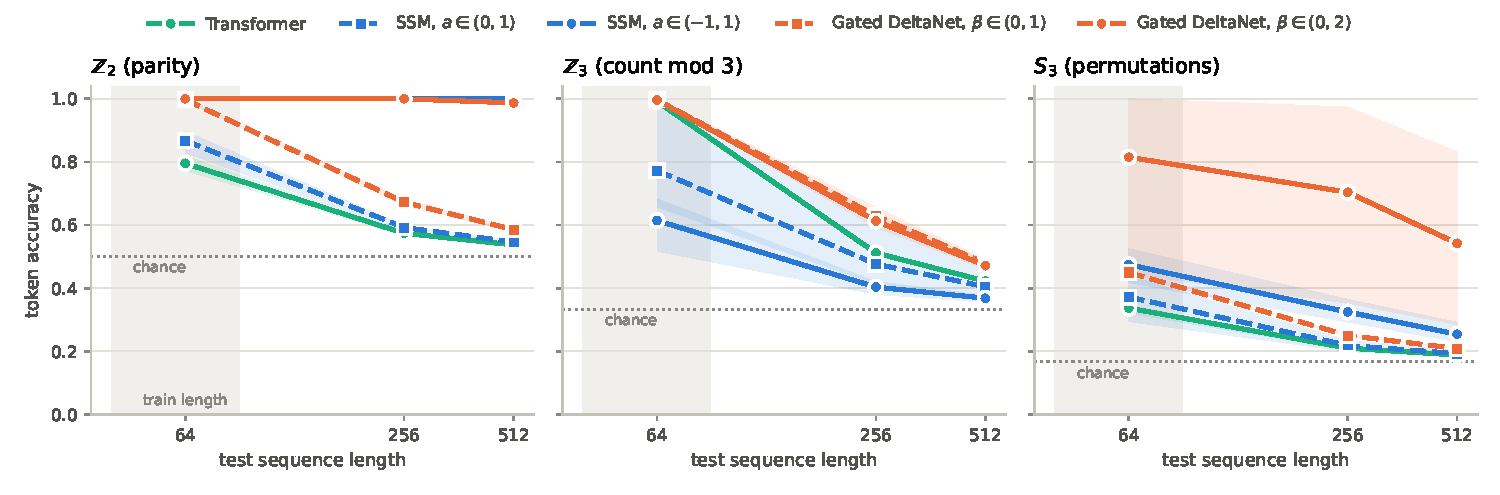
\includegraphics[width=\linewidth]{figures/state_tracking}
\caption{Length generalisation on state tracking. Colour = architecture family, line style =
eigenvalue range (dashed/square: positive only; solid/circle: extended to negative). Only models whose
transitions can represent the group keep their accuracy beyond the training length (grey band). Lines: mean over 3 seeds; shading: min--max.}
\label{fig:state}
\end{figure}

\paragraph{Beyond negative eigenvalues (RQ2b).} Table~\ref{tab:state} (bottom block) and
Fig.~\ref{fig:state-ext} add the rotational SSM and DeltaProduct$_2$.
\todo{Interpret: DeltaProduct$_2$ with $\beta\in(0,2)$ is the only model that learns $S_3$ on all 3
seeds and keeps 0.91 at 8$\times$ the training length (Gated DeltaNet: 0.54, high variance). On
$\mathbb{Z}_3$, every model that fits the training length (attention, DeltaNet, DeltaProduct, rotational
SSM: 0.97--1.00) falls to 0.43--0.52 at length 512. The rotational SSM fits $\mathbb{Z}_2$ at length 64
on only 1 of 3 seeds.}

\begin{figure}[h]\centering
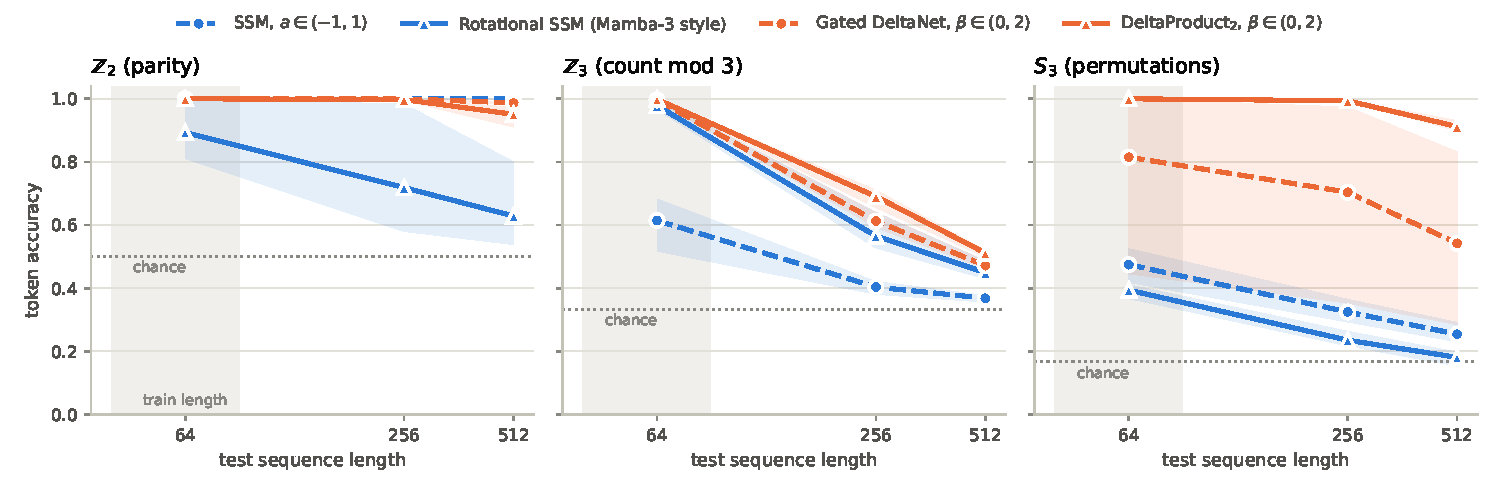
\includegraphics[width=\linewidth]{figures/state_tracking_ext}
\caption{The extensions against their predecessors (dashed). Lines: mean over 3 seeds; shading: min--max.}
\label{fig:state-ext}
\end{figure}

\begin{table}[h]\centering\small
\begin{tabular}{lccccc}
\toprule
Train length & test 16 & test 32 & test 64 & test 256 & test 512 \\
\midrule
16 & 1.000$\pm$0.000 & -- & 0.675$\pm$0.187 & 0.432$\pm$0.065 & 0.382$\pm$0.032 \\
32 & -- & 0.995$\pm$0.008 & 0.877$\pm$0.127 & 0.518$\pm$0.093 & 0.425$\pm$0.046 \\
64 & -- & -- & 0.719$\pm$0.186 & 0.453$\pm$0.081 & 0.394$\pm$0.040 \\
\bottomrule
\end{tabular}

\caption{Rotational SSM on $\mathbb{Z}_3$ trained at different lengths (mean $\pm$ std over 3 seeds).}
\label{tab:rotation-length}
\end{table}

\begin{figure}[h]\centering
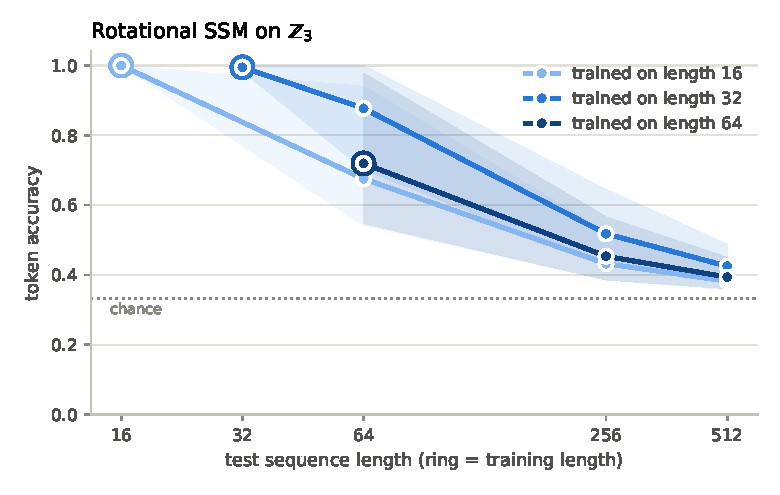
\includegraphics[width=0.6\linewidth]{figures/rotation_length}
\caption{Rotational SSM on $\mathbb{Z}_3$: accuracy vs.\ test length for three training lengths.
Ring: the training length. Shading: min--max over 3 seeds.}
\label{fig:rotation-length}
\end{figure}

\todo{Table: RQ1 MQAR accuracy vs.\ number of pairs (with state size column).}
\todo{Table: RQ3 hybrid placement.}
\todo{Table: RQ4 latency / memory / decode throughput on the RTX 4050.}
\todo{Interpret every table in prose.}

\section{Qualitative Results}
\label{sec:qual}
% Guideline 2.10: visualisations with meaningful captions, discussed in the text.
\todo{Figures:
(i) accuracy vs.\ position for parity (where does the positive-decay SSM lose track?);
(ii) attention map of the Transformer on MQAR (the induction pattern) vs.\ the SSM's implicit
     attention matrix $L\odot CB^\top$;
(iii) SSM state norm / sign over time on a parity sequence, with and without negative eigenvalues;
(iv) MQAR recall accuracy vs.\ number of pairs (capacity curve);
(v) latency and memory vs.\ sequence length.}

\section{Analysis and Discussion}
\label{sec:discussion}

\paragraph{Why the methods perform as they do.} The results follow the two mechanisms of
Section~\ref{sec:theory} closely. For \emph{state tracking} what matters is which transitions the recurrence can
express, not how large the state is: all recurrent models had the same 8192-float state, and the outcome was
decided by the eigenvalue range and by whether the transition can be non-diagonal. For \emph{recall} what matters
is how much the state can hold and how efficiently it is used: attention never runs out of memory, the SSM breaks
at a point that moves with its state size, and the delta rule postpones the break by overwriting instead of
accumulating. No single recurrent model is best at both, and attention is best at recall but fails to
generalise on state tracking. This is the empirical case for the hybrid architectures used in practice.

\paragraph{Failure case 1: recall beyond state capacity.} The SSM with $N=16$ solves 16 pairs (0.991) but reaches
only 0.134 with 32 pairs, and the $N=64$ model fails at 64 pairs (0.053). The failure is abrupt rather than
gradual, and its position moves with the state size, which identifies capacity as the cause. A caveat: ``failed
within 20{,}000 steps'' bounds what was learned, not what is learnable, and one seed was used per configuration.
That the breaking point moves monotonically with $N$ supports the capacity explanation over an optimisation
accident.

\paragraph{Failure case 2: shortcuts that fit the training length.} Gated DeltaNet with $\beta\in(0,1)$ reaches
0.997 on parity at length 64 but only 0.586 at 512. By the proposition of Section~\ref{sec:math} its transitions
cannot implement a sign flip, so its near-perfect training-length accuracy must come from a solution that exploits
the limited length, for example by counting within a bounded window. The same holds for the Transformer on
$\mathbb{Z}_3$ (0.991 vs.\ 0.422). In-distribution accuracy alone would have suggested these models learned the
task; only the length-generalisation test reveals otherwise.

\paragraph{Failure case 3: expressible but not learned (rotational SSM on $\mathbb{Z}_3$).} The rotational SSM can
represent $\mathbb{Z}_3$ exactly; a unit test confirms that a rotation by $2\pi/3$ returns the state after three
steps. Yet training never finds this solution. It fits short sequences (1.000 at length 16), becomes unreliable at
length 64 (0.719, two of three seeds fail), and never generalises (at most 0.43 at 512). The learned weights
(Figure~\ref{fig:rotation-angles}) show why: the angles are not multiples of $120^\circ$, tokens 1 and 2 receive
nearly identical angles, and part of the memory decays, so the network built a short-range shortcut. We see two
reasons why gradient descent struggles here. First, the loss depends on the angle $\theta$ through terms like
$\cos(k\theta)$ for all $k\le T$, so the loss surface in $\theta$ oscillates more rapidly the longer the training
sequences are; this matches the drop in training-length accuracy from 1.000 to 0.719 as $T$ grows from 16 to 64.
Second, the target angle $2\pi/3$ is an interior value that must be hit exactly, because any error accumulates over
the sequence. In contrast, a sign flip is reached by pushing the decay towards $-1$, and a reflection by pushing
$\beta$ towards 2; these are saturating parametrisations that gradient descent approaches exponentially fast.

\paragraph{Failure case 4: $\mathbb{Z}_3$ resists every model, although $S_3$ does not.} DeltaProduct with
$\beta\in(0,2)$ generalises on $S_3$ (0.912 at length 512) but not on $\mathbb{Z}_3$ (0.511), even though
$\mathbb{Z}_3$ is a subgroup of $S_3$ (its rotations). We offer a tentative explanation in line with failure case 3.
In $S_3$, the three transpositions can be implemented by single exact reflections ($\beta\to 2$, saturating), and
the 3-cycles then arise automatically as products of two such reflections. In $\mathbb{Z}_3$, every non-identity
token must itself be a rotation by exactly $\pm120^\circ$, which requires the two keys of the token to be at
exactly $60^\circ$ to each other, an interior value again. Testing this hypothesis, for example by initialising
the keys at the required angle or by training with a length curriculum, is left for future work.

\paragraph{Methodology lesson: an insufficient training budget ranks models wrongly.} Our first recall sweep
(length 512, vocabulary 4096, 4000 steps) produced unusable results: even attention reached only 0.12--0.30
with 8 pairs, and accuracy was non-monotonic in the number of pairs (e.g.\ the $N=64$ SSM scored 0.41 with 8 pairs
but 0.99 with 16). Recall is learned in a sudden jump after a plateau, so a small fixed budget measures whether a
run happened to jump in time, not what the model can do. Checks on the CPU excluded two other explanations (a
short convolution for attention, a smaller vocabulary). A calibration run with up to 20{,}000 steps and early
stopping then gave every model at least 99\% on 16 pairs, with steps-to-90\% of 500 (attention + short conv), 1500
(Gated DeltaNet), 5500 (SSM) and 6500 (plain attention). The final recall study uses this budget.

\paragraph{Hyperparameter sensitivity.} Three sensitivities stood out. (i) A short causal convolution, which gives
each layer direct access to the previous few tokens, makes attention learn recall about 13$\times$ faster (500 vs.\
6500 steps); without it attention must first learn a separate previous-token mechanism. (ii) In a preliminary CPU
experiment, attention with one 64-dimensional head reached 91\% on a small recall task while the same model with
two or four narrower heads stalled near 53\%; we therefore used a single head for recall. (iii) The random seed
matters for the harder state-tracking cases: Gated DeltaNet with $\beta\in(0,2)$ on $S_3$ ranges from 0.28 to 0.83
at length 512 across seeds, and the rotational SSM solves parity on one seed out of three. Reporting three seeds
was therefore necessary; a single seed would have supported opposite conclusions.

\paragraph{Ablations.} The experiments double as ablations of single mechanisms with everything else fixed: the
eigenvalue range (SSM and DeltaNet, Table~\ref{tab:state}), rotational transitions, one versus two Householder steps
per token, the training length of the rotational SSM (Table~\ref{tab:rotation-length}), the state size of the SSM
(Table~\ref{tab:recall}) and the short convolution in attention.

\paragraph{Computational requirements.} Every model trains on a 6\,GB laptop GPU in minutes. At the lengths that
fit, however, the fused FlashAttention kernel \citep{dao2022flashattention} beats our linear-time layers, whose
asymptotic advantage would only show beyond roughly 32k tokens. The quality of the GPU kernel matters as much as
the complexity class, which is why production SSMs ship hand-written kernels. Our Triton kernel illustrates the
difficulty. It is faster and leaner than the PyTorch code but reaches only about 5\% of the GPU's memory
bandwidth. It is neither compute-bound nor bandwidth-bound but latency-bound: the loop over time is strictly
sequential and only $b\cdot H\cdot P/B_P = 64$ programs run in parallel, too few to hide memory latency on 20
streaming multiprocessors. This is precisely the motivation for Mamba-2's chunked algorithm, which turns most of
the scan into matrix multiplications that can use tensor cores; a Triton version of Algorithm~\ref{alg:scan} is
the natural next step. In generation, the recurrent models' constant state saves memory (32\,MB vs.\ 512\,KB per
layer at 8k tokens), but per-token latency at batch 4 is dominated by kernel-launch overhead.

\paragraph{Limitations.} The models are small (two layers, under half a million parameters) and the tasks are
synthetic, so the results characterise mechanisms rather than language-modelling quality. Recall results use one
seed. The Triton kernel implements only the forward pass, so training used the PyTorch chunked algorithm. The
benchmarks were taken on a laptop GPU whose clock varies with load and temperature; the scan table therefore
reports only lengths of at least 4k tokens, where timings were stable. Finally, our rotational SSM uses a
simplified version of the Mamba-3 parametrisation (angles from a separate projection, Euler-style input term), and
may behave differently from the original.

\section{Conclusion}
\label{sec:conclusion}

This project asked what a fixed-size, fading memory costs a sequence model and what fixes it, using
from-scratch implementations of attention, a selective SSM, Gated DeltaNet and two recent extensions, all trained
on one laptop GPU.

\paragraph{What was learned.} The two abilities studied fail for different reasons and are fixed by different
means. State tracking is limited by \emph{expressivity}: with positive real transitions no model learns parity
beyond the training length, a single change to negative eigenvalues makes the SSM solve it at 8$\times$ the
training length (0.999), and DeltaProduct, whose transitions are products of two reflections, is the only model
that learns the non-abelian group $S_3$ reliably (0.912 at 8$\times$ the training length, all seeds). Recall is
limited by \emph{capacity}: the SSM breaks once the number of stored pairs outgrows its state, a larger state moves
the breaking point, and the delta rule stores 64 pairs with half the state of an SSM that fails. Attention solves
recall trivially but does not generalise on state tracking.

\paragraph{Strengths and limitations.} The comparison is controlled (one codebase, matched state sizes, three
seeds for state tracking), the algorithms are verified against reference recurrences, and the failure cases are
backed by evidence including the learned weights themselves. The main limitations are the small scale, the
synthetic tasks and a single seed for recall.

\paragraph{The broader lesson.} Being able to represent a solution is not the same as learning it. The
rotational SSM can represent counting modulo 3 but learns a shortcut; several models fit the training length
perfectly without learning the rule; and a too-short training budget once ranked the models in the wrong order.
Each of these was caught only by testing beyond the training distribution or by looking inside the model.

\paragraph{Future work.} Natural next steps are a length curriculum or targeted initialisation to test whether
the rotational SSM and DeltaProduct can be made to learn $\mathbb{Z}_3$; a chunked Triton kernel with a backward
pass, to turn the linear-time recurrences into an actual speed advantage on the GPU; more seeds for the recall
study; and hybrid models that combine a few attention layers for recall with DeltaProduct layers for state
tracking, evaluated on natural language.


\bibliographystyle{plainnat}
\bibliography{refs}
\end{document}
